\section{Analysis}
\label{section:eval}

This section details the evaluation of INFLEX as well as details pertaining to its implementation.
A reference implementation of the inflector was developed as a component of the POX network controller \cite{pox}.
Additionally, INFLEX support for \ac{TCP} was added to the Linux kernel, and is available as a small patch for version 3.8.
All source code, as well as a virtual machine to replicate subsequent tests, is being made publicly available.
The use of POX in particular invalidates any rigorous performance evaluation, as the implementation is not geared towards efficiency.
Instead, the contributed code acts as a proof-of-concept for INFLEX, allowing the mechanics of the specification to be inspected and fine-tuned.

\begin{figure}
    \begin{subfigure}[b]{1.0\linewidth}
        \centering
        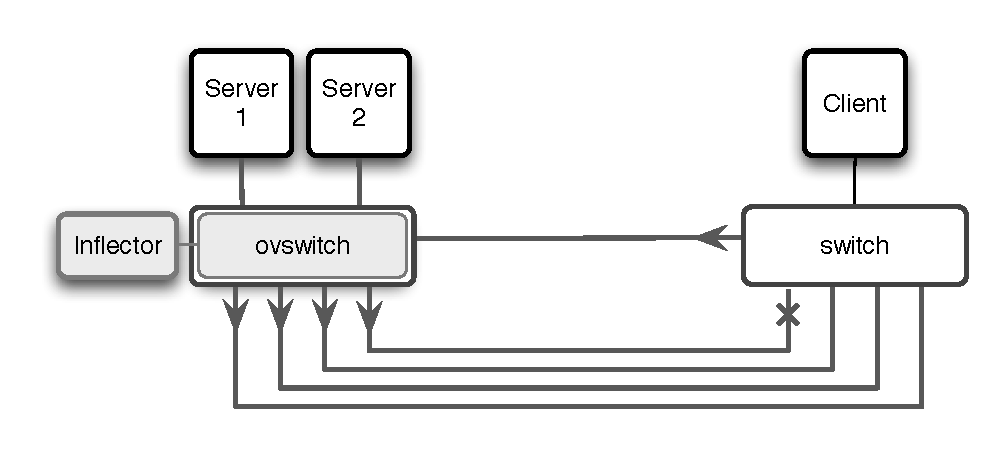
\includegraphics[width=4.0in]{figures/inflex/simtopo.eps}
    \end{subfigure}%
    \caption{Simulation setup. \label{fig:simtopo}}
\end{figure}

To this end, a simple evaluation scenario is used, illustrated in figure \ref{fig:simtopo}.
On one end is an INFLEX capable domain: a set of virtual hosts acting as \emph{servers} connected to an Openvswitch edge switch controlled by an inflector.
On the other end is a remote \emph{client}.
Typically this is an end-user device outside network operator control. We assume that the client is running a legacy network stack and connected to a switch with no \ac{SDN} functionality.
A single physical connection between the client and this switch acts as the bottleneck for all flows, with the bandwidth set to 10Mb/s. The edge switch has four potential planes over which it can forward traffic between the \emph{servers} and the \emph{client}. We simulate failures within the INFLEX domain by artificially dropping all forwarded packets belonging to a given plane; we denote this plane as being \emph{down}. At any given moment one of the four available planes is down; each such simulated failure lasts for 15 seconds at a time, affecting planes cyclically.
The reverse path, connecting from client to server, is always assumed to be functional.
Propagation delay between both switches is set to $50$ms, resulting in a base round trip time between servers and client of $100$ms.

\subsection{Sender-side resilience}

The first case study under review is one of the most common use cases for datacenters: a remote client \emph{downloading} data from hosted servers.
Under the conditions described previously, the forwarding path will be periodically affected by recurring failures.
Since the nature and the origin of the fault are not always apparent to network devices, it is assumed that network elements within the INFLEX domain have no indication of the ongoing failure.
Instead, it is up to the servers to detect and recover from perceived problems by issuing inflection requests.
Clearly, requesting a path incurs some cost to network and host alike.
For the network, an inflection request requires additional processing.
For the host, this processing manifests itself as increased delay.
This begs the question: when should a host request an inflection?
The obvious candidate is to piggyback inflection requests on retransmissions spawned by \ac{RTO}.
This leverages an existing transport mechanism which is well understood and only triggered under anomalous path conditions (as opposed to congestive losses).
From the perspective of the host, any delay incurred by the inflection request is amortized by the retransmission timeout itself, which has a minimum value of 1 second.
From the perspective of the network, such inflection requests should be both rare, reducing the amount of processing required, and critical to improve availability, justifying the expense in addressing them.

\begin{figure}
    \begin{subfigure}[b]{1.0\linewidth}
        \centering
        \includegraphics[width=5.0in]{figures/inflex/sender-legacy.pdf}
        %\caption{Legacy server\label{fig:legacy-sender}}
    \end{subfigure}%

    \begin{subfigure}[b]{1.0\linewidth}
        \centering
        \includegraphics[width=5.0in]{figures/inflex/sender-inflex.pdf}
        %\caption{INFLEX server\label{fig:inflex-sender}}
    \end{subfigure}%
    \caption{Congestion window for concurrent downloads towards client from legacy (above) and INFLEX (below) servers.
\label{fig:sender}}
\end{figure}

Figure \ref{fig:sender} displays the congestion window over time for two concurrent flows towards a remote client.
The first connection traced is a download from a server without INFLEX support, in which all packets are forwarded over the default path.
The vertical lines signal the points at which the default forwarding path, plane $0$, fails.
Despite only failing for $15$sec, the disruption to the transport flow lasts twice as long due to the exponential nature of the retransmission timeout, which doubles in duration at each occurrence.
The second connection traced is a download occurring in parallel from an INFLEX capable server. 
In this case, each path failure is recovered by sending an inflection request on each retransmission timeout.
The returned path is randomly assigned, as our basic proof-of-concept inflector does not currently keep track of network conditions.
The time between path failure and flow recovery is directly tied to the \ac{RTO}, in this case taking approximately one second. 
This value cannot be improved upon within the INFLEX framework, as the duration of flow entries introduced by inflection requests has a minimum timeout of 1 second.
Conveniently however, this matches the lower bound of the \ac{RTO} as defined by \ac{TCP}, and it is therefore unlikely that a transport protocol would desire faster fail-over.
In practice, the recovery time may be extended in order to account for spurious timeouts.
For connections over wireless media in particular, timeouts may occur due to transient effects such as interference.
While this is functionally equivalent to path failure, the transient nature of such events does not always require changes to the forwarding path.

An interesting implication of figure \ref{fig:sender} is that \textbf{\ac{TCP} senders using INFLEX can accommodate path fail-over seamlessly}.
Retransmissions conveniently distinguish between congestion events, triggering fast retransmission and similar heuristics, and pathological network conditions, which spawn repeated retransmission timeouts.
In the case of the latter, the adopted response is to reset the congestion window and resume slow start -- effectively restarting the flow.
This behaviour is extremely conservative, but is a natural corollary of assuming as little as possible about the underlying network.
As a result, no substantial change is required to the congestion control mechanisms employed by \ac{TCP} in retrofitting cross-layer path fail-over at the sender using INFLEX.

\subsection{Receiver-side resilience}

Path failures can also affect the reverse path with equally nefarious consequences: the sender will repeatedly timeout in the absence of acknowledgements from the receiver.
Unlike failures affecting the forward path however, the INFLEX host does not actively track the reliability of the ongoing connection.
\ac{TCP} is sender driven, with receivers primarily generating acknowledgements as a response to inbound data. 
Hence, the reverse path lacks the reliable delivery mechanisms available in the forward path; if the \emph{\ac{TCP} Timestamp} option is not used, the receiver often lacks even an accurate RTT estimate.
Furthermore, in the absence of data packets to be sent, there is no \ac{RTO} on which to trigger inflection requests.

\begin{figure}
    \begin{subfigure}[b]{1.0\linewidth}
        \centering
        \includegraphics[width=5.0in]{figures/inflex/recv-cwnd.pdf}
    \end{subfigure}
    \caption{Concurrent uploads from client towards servers.\label{fig:receiver}}
\end{figure}

\begin{figure}
    \begin{subfigure}[b]{1.0\linewidth}
        \centering
        \includegraphics[width=5.0in]{figures/inflex/recv-legacy.pdf}
    \end{subfigure}
    \begin{subfigure}[b]{1.0\linewidth}
        \centering
        \includegraphics[width=5.0in]{figures/inflex/recv-inflex.pdf}
    \end{subfigure}%
    \caption{Data packet inter-arrival time for legacy (above) and INFLEX (below) receivers.\label{fig:inter-arrival-time}}
\end{figure}

A receiver must instead rely on inferring path failure from the packet inter-arrival time when generating duplicate acknowledgements.
With the exception of cases where immediate receiver feedback is required, such as a \ac{TCP} timestamp request, duplicate acknowledgements are typically sent on the arrival of out-of-order data.
Under path failure, the arrival time between such out-of-order events will rise exponentially as the sender \ac{TCP} stack becomes tied to its own retransmission timeout.
This behaviour is illustrated in figures \ref{fig:receiver} and \ref{fig:inter-arrival-time}, which show the result of using INFLEX with the same experimental setup but a reversed flow of data.
Figure \ref{fig:receiver} displays the evolution of the congestion window size over time as the client uploads data concurrently to both a legacy and an INFLEX server.
While the single forwarding path does not experience outages, the reverse path is periodically affected by failures.
The corresponding data packet inter-arrival time is shown in figure \ref{fig:inter-arrival-time}, with each sample point also displaying the routing plane used.
For an ongoing \ac{TCP} flow with sufficient data from the application layer the packet inter-arrival time at the receiver should be consistently low.
RTT level dynamics are apparent on slow start, in which the sender is clocked by incoming \acp{ACK}, and during congestion events, in which out-of-order delivery temporarily affects the throughput.
On path failure however, the inter-arrival time increases exponentially, with each inbound packet triggering a duplicate acknowledgement.
For the upload to the legacy server, successive \acp{RTO} result in a recovery time of nearly $30$sec.

An INFLEX receiver can use this information to decide when to trigger an inflection request. 
It can achieve this by setting a threshold for the time elapsed between duplicate acknowledgements, henceforth referred to as $dupthresh$.
Comparatively to the sender, the receiver should be more conservative, as by design it has less information on which to act upon and does not typically exert control on the congestive feedback loop.
Furthermore, neither sender nor receiver can reliably detect whether the forward or reverse path are at fault.
By acting conservatively, a receiver allows the sender, which may also be INFLEX capable, to initiate recovery before trying to correct the reverse path.
For the experiment displayed in figure \ref{fig:inter-arrival-time}, the $dupthresh$ is set to twice the \ac{RTO}, resulting in an overall downtime of approximately 3 seconds.
Since each data point is generated on inbound data packets, recovery is signalled by a packet pair.
A first inbound packet exceeding $dupthresh$ triggers an inflection request, which piggybacks on the acknowledgement sent out in response.
A second inbound packet returns approximately 1 RTT later with the forwarding plane assigned by the network attached.
Clearly some failures may not be recoverable, particularly if the remote host is not INFLEX capable and the fault lies on the reverse path.
Nonetheless, the overhead incurred at the host is negligible, merely complementing congestion avoidance mechanisms with additional signalling.
Remarkably, INFLEX incurs no additional memory costs at the host, operating as an extended \ac{API} over the existing $inet\_connection$ socket, rendering it equally applicable to all transport protocols which use this socket structure, such as \ac{SCTP} and \ac{DCCP}.

\subsection{Network overhead}

\begin{figure}
    \begin{subfigure}[b]{1.0\linewidth}
        \centering
        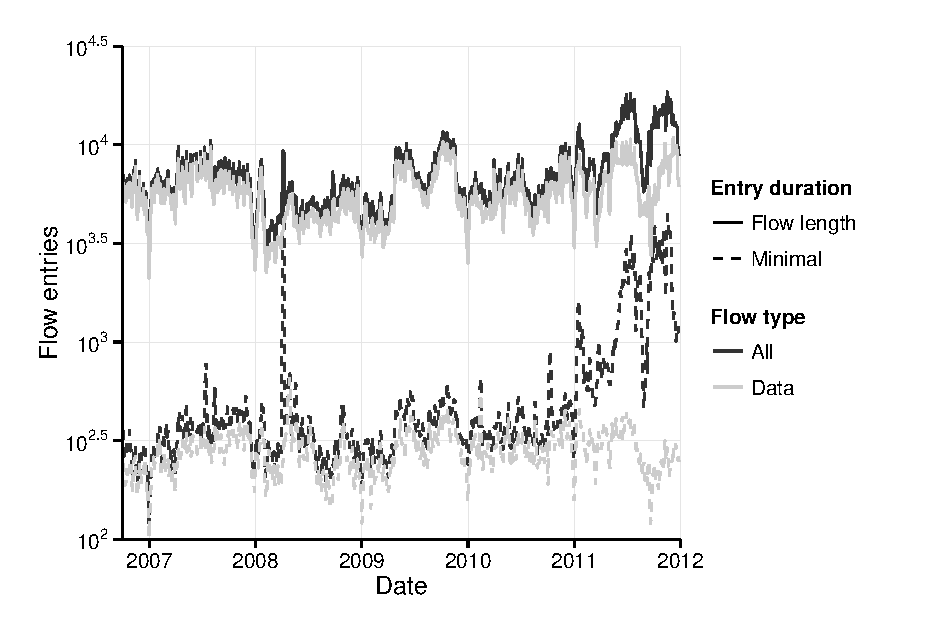
\includegraphics[width=5.0in]{figures/inflex/flow.eps}
    \end{subfigure}%
    \caption{Mean flow state for outbound traffic\label{fig:flow}}
\end{figure}

The granularity at which an \ac{SDN} deployment should manage traffic is often subject to debate.
On one hand, hardware advances such as \acp{TCAM} offer fast lookup times over large tables, affording flow precision for many potential \ac{SDN} deployments.
On the other, deployments will often include cheaper, more flexible software switches which are less capable of scaling performance with the number of flow entries.
Importantly, operating on a per-flow granularity is more likely to overload the controller, which itself can be a considerable source of latency.
As a result, managing flow aggregates is often the preferred means of reducing this overhead, at the cost of flexibility in affecting flows individually.

INFLEX does neither strictly, exerting network control at a sub-flow granularity while pushing flow state to the end-host.
Figure \ref{fig:flow} investigates the relative expected overhead incurred by the network on adopting such an architecture.
The graph tracks the mean flow state from applying different flow entry policies for outbound traffic in the MAWI dataset.
The solid lines track the resulting flow table size if traditional per-flow state were maintained, with every unique five tuple inserting a table entry for the entirety of the flow's lifetime.
This is equivalent to the mean number of flows at the observed link and is further refined according to whether data was traced for the unique five tuple.
For domains which exchange traffic with the wider Internet, per-flow state can be particularly crippling as malicious SYN floods and port scans regularly inflate the required state in the network.
Such attacks had visible impact in 2011 in particular, nearly doubling the number of flows.

INFLEX however inserts ephemeral rules in response to inflection requests.
For the worst possible case, all existing flows would trigger an inflection request simultaneously -- matching the overhead incurred by a per-flow approach.
In practice even this is overly pessimistic, as an inflector could resort to a per-aggregate granularity in the case of widespread outages.
Actual network state would strongly depend on the exact inflection strategy adopted by the transport protocol.
One practical reference point is to investigate the resulting overhead if paths were requested on flow start, as this number will exceed retransmission timeouts under normal operating conditions.
This is further illustrated in figure \ref{fig:flow}, which also tracks flow table size if each unique five tuple were to only generate a flow entry for 1 second, the minimum expiry time for Openflow.
This is functionally equivalent to the flow arrival rate, and determines the expected number of requests per second sent to the controller.
The resulting flow table size is reduced dramatically in comparison to the traditional case where state is allocated for the duration of the flow, and the order of magnitude difference is crucial for software switches in particular.
However, under such conditions state becomes more strained by the large fluctuations imposed by \ac{DOS} attacks, suggesting that inflection requests should only be used after connection establishment; this corresponds to the grey dotted line in figure \ref{fig:flow}. Importantly, such an approach also opens the possibility of using inflection requests for assisting traffic management in addition to enabling improved resilience.

%However, a host might wish to issue an inflection request for purposes other than resilience.
%In most cases flow entries are only issued to enforce a decision by the local controller. 
%In trusted environments such as data centres, this state could potentially be pushed back to the host, reducing the resulting flow table size for intermediate network elements.
%Figure \ref{fig:flow} investigates the potential gains of such an approach by reducing the flow entry duration to 1 second -- the minimum entry duration imposed by Openflow.

%Flow-based matching is unfortunately unable to know the nature of the flow \emph{a priori}: all unique five-tuples will be forwarded to the controller independently of the size of the flow.
%This is particularly crippling for domains which exchange traffic with the wider Internet, and are therefore subjected to malicious SYN floods and port scans on a regular basis.
%Figure \ref{fig:flow} investigates the mean number of flow entries which would result for outbound traffic in the MAWI dataset if each unique five-tuple were to be inserted into a flow table for differing periods of time.
%The solid lines track flow table size if each entry spans the entirety of a flow's lifetime, rounded up to the closest second.
%The topmost line takes into account all unique five-tuples, and provides a baseline for applying traditional per-flow methods to the MAWI dataset.
%The grey line beneath shows the reduction in flow entries which could be achieved if the controller were to act only upon flows over which data is exchanged -- effectively ignoring unestablished connections.
%Both are on the same order of magnitude despite the number of unestablished connections increasing significantly in 2011 as a result of DOS attacks.


%\section{Discussion?}
%
%However, a host might wish to issue an inflection request for purposes other than resilience.
%This may include selecting a path on flow start in order to balance traffic, as proposed in \cite{me}, or search for the forwarding plane providing the lowest latency to a given destination.
%Such occurrences are left for future work, but are accounted for through the Exposure bit.
%This final bit of the INFLEX header is set on every retransmission, serving two purposes.
%Foremost, it exposes the amount of congestion a host experiences, and can be used by the network in assessing performance across different overlays.
%Finally, it allows the network to infer the nature of the inflection request, and whether a host is switching path due to a potential failure.
%

